\section{Условия труда}
В настоящем разделе будут рассмотрены условия, в которых
находился работник при разработке программного обеспечения.

\subsection{Анализ опасных и вредных факторов при разработке программного
    обеспечения и мероприятия по их устранению}

Разработка программного обеспечения требует постоянного взаимодействия с
вычислительными машинами, что связано с воздействием ряда вредных и зачастую опасных факторов, таких
как статическое электричество, рентгеновское излучение, электромагнитные поля,
ультрафиолетовое излучение, блики, отраженный свет и мерцание изображения.
Рассмотрим более подробно некоторые из вышеуказанных факторов.

\subsubsection{Микроклимат}

Работа за компьютером не требует серьезных физических усилий, поэтому ее относят к категории \textit{1а}.
Оптимальные нормы микроклимата для этой категории определяются таблицей \textit{СанПиН 2.2.2/2.4.1340-03}
(таблица~\ref{tables:microclimate}).

\begin{table}[hbt!]
\begin{tabu}[\textwidth]{|X[c]|X[c]|X[c]|X[c]|}
    \hline
    & Температура воздуха,~\celsius & Относительная влажность воздуха,~\% & Скорость движения воздуха, $ м/с $ \\
    \hline
    Холодный & 22-24 & 40-60 & 0.1 \\
    \hline
    Теплый & 23-25 & 40-60 & 0.1 \\
    \hline
\end{tabu}
\caption{Оптимальные нормы микроклимата}
\label{tables:microclimate}
\end{table}

Вредным фактором при работе с ЭВМ является также запыленность помещения. Этот фактор усугубляется влиянием на частицы пыли
электростатических полей персональных компьютеров.

Для устранения несоответствия параметров указанным нормам проектом предусмотрено использование системы кондиционирования как
наиболее эффективного и автоматически функционирующего средства.

Нормы \textit{СанПиН 2.2.4.1294-03} <<Санитарно-гигиенические нормы допустимых уровней ионизации воздуха>> определяют уровни положительных и
отрицательных ионов в воздухе (таблица~\ref{tables:gigenic}):

\begin{table}[hbt!]
\begin{tabu}[\textwidth]{|X[c]|X[c]|X[c]|}
    \hline
    \multirow{2}{*}{Уровни} & \multicolumn{2}{c|}{Число ионов в 1 см куб. воздуха} \\
    \cline{2-3}
    & $ n^+ $ & $ n^- $ \\
    \hline
    Минимально необходимые & 400 & 600 \\
    \hline
    Оптимальные & 1500-3000 & 3000-5000 \\
    \hline
    Предельно допустимые & 50000 & 50000 \\
    \hline
\end{tabu}
\caption{Уровни ионизации воздуха помещений при работе на ВДТ и ПЭВМ}
\label{tables:gigenic}
\end{table}

Для обеспечения требуемых уровней предусмотрено использование системы ионизации \textit{Сапфир-4А}.

Концентрация вредных химических веществ в помещениях с ПЭВМ не должна превышать <<ПДК загрязняющих веществ в атмосферном воздухе
населенных мест>> \textit{ГН 2.1.6.789-99}. Для выполнения указанных требований предусмотрено применение фильтров из активированного угля.

\subsubsection{Шум и вибрации}

Уровень шума на рабочем месте программиста не должен превышать 50 дБА, а уровень вибрации не должен превышать допустимых норм
вибрации. \textit{СанПиН 2.2.2.542-96} устанавливает следующие нормы на вибрацию (таблица \ref{tables:vibration}).
\begin{table}[hbt!]
\begin{tabu}[0.8\textwidth]{|X[c]|X[c]|X[c]|}
    \hline
    Среднегеометрические & \multicolumn{2}{c|}{Допустимые значения} \\
    частоты октавных полос, Гц & \multicolumn{2}{c|}{по виброскорости} \\
    \cline{2-3}
    & $ \times 10, м/с $ & $ дБ $ \\
    \hline
    2 & 4.5 & 79 \\
    \hline
    4 & 2.2 & 73 \\
    \hline
    8 & 1.1 & 67 \\
    \hline
    16 & 1.1 & 67 \\
    \hline
    31.5 & 1.1 & 67 \\
    \hline
    63 & 1.1 & 67 \\
    \hline
    Корректированные значения и их уровни & 2.0 & 72 \\
    \hline

\end{tabu}
\caption{Допустимые нормы вибрации на рабочих местах с ВДТ и ПЭВМ}
\label{tables:vibration}
\end{table}

При разработке программного обеспечения внутренними источниками шума являются вентиляторы, а также принтеры и другие периферийные
устройства ЭВМ. 

Внешние источники шума -- прежде всего, шум с улицы и из соседних помещений. Постоянные внешние источники шума, превышающего нормы,
отсутствуют.

Для устранения превышения нормы проектом предусмотрено применение звукопоглощающих материалов для облицовки стен и потолка
помещения, в котором осуществляется работа с вычислительной техникой.

\subsubsection{Освещение}
Наиболее важным условием эффективной работы программистов и пользователей является соблюдение оптимальных параметров системы
освещения в рабочих помещениях.

Естественное освещение осуществляется через светопроемы, ориентированные в основном на север и северо-восток (для исключения
        попадания прямых солнечных лучей на экраны компьютеров) и обеспечивает коэффициент естественной освещенности (КЕО) не ниже
1,5\%.

В качестве искусственного освещения проектом предусмотрено использование системы общего равномерного освещения. В соответствии с
\textit{СанПиН 2.2.2/2.4.1340-03},  освещенность на поверхности рабочего стола находится в пределах 300-500 лк. Разрешается использование
светильников местного освещения для работы с документами (при этом светильники не должны создавать блики на поверхности экрана).

Правильное расположение рабочих мест относительно источников освещения, отсутствие зеркальных поверхностей и использование матовых
материалов ограничивает прямую (от источников освещения) и отраженную (от рабочих поверхностей) блескость. При этом яркость
светящихся поверхностей не превышает 200 кд/кв.м, яркость бликов на экране ПЭВМ не превышает 40 кд/кв.м, и яркость потолка не
превышает 200 кд/кв.м.

В соответствии с \textit{СанПиН 2.2.2/2.4.1340-03}  проектом предусмотрено использование люминесцентных ламп типа ЛБ в качестве источников
света при искусственном освещении. В светильниках местного освещения допускается применение ламп накаливания.

Применение газоразрядных ламп в светильниках общего и местного освещения обеспечивает коэффициент пульсации не более 5\%.
Таким образом, проектом обеспечиваются оптимальные условия освещения рабочего помещения.

\subsubsection{Рентгеновское излучение}
В соответствии с \textit{СанПиН 2.2.2/2.4.1340-03}, проектом предусмотрено использование ПЭВМ, конструкция которых обеспечивает мощность
экспозиционной дозы рентгеновского излучения в любой точке на расстоянии 0,05 м. от экрана и корпуса монитора не более 0,1
мбэр/час (100 мкР/час). Результаты сравнения норм излучения приведены в таблице \ref{tables:rentgen}.

\begin{table}[hbt!]
\begin{tabu}[\textwidth]{|X[c]|X[c]|}
    \hline
    & Допустимое значение, $ мкР/час $, не более \\
    \hline
    СанПиН 2.2.2/2.4.1340-03 & 100 \\
    \hline
    TCO-99 & 500 \\
    \hline
    MPR II & 500 \\
    \hline
\end{tabu}
\caption{Сравнение норм рентгеновского излучения в различных стандартах}
\label{tables:rentgen}
\end{table}

Как видно из таблицы \ref{tables:rentgen}, стандарты \textit{MPR II} и \textit{TCO-99} предъявляют менее жесткие требования к
рентгеновскому излучению, чем СанПиН. Но
при соблюдении оптимального расстояния между пользователем и монитором дозы рентгеновского излучения не опасны для большинства
людей.

\subsubsection{Неионизирующие электромагнитные излучения}

В соответствии с \textit{санпин 2.2.2/2.4.1340-03}, допустимые значения параметров неионизирующих излучений приводятся в таблицах
    \ref{tables:electric} и \ref{tables:magnet}.
\begin{table}[Hbt!]
\begin{tabu}[\textwidth]{|X[c]|X[c]|}
    \hline
    Диапазон частот, $ \times 10^3 $, гц & Допустимые значения, $В/м$ \\
    \hline
    $ 5 \times 10^{-3}$ --- 2 & 25 \\
    \hline
    2 --- 400 & 2.5 \\
    \hline
\end{tabu}
\caption{Предельно допустимые значения напряженности электрического поля}
\label{tables:electric}
\end{table}

\begin{table}[Hbt!]
\begin{tabu}[\textwidth]{|X[c]|X[c]|}
    \hline
    Диапазон частот, $ \times 10^3 $, гц & Допустимые значения, $нТл$ \\
    \hline
    $ 5 \times 10^{-3}$ --- 2 & 250 \\
    \hline
    2 --- 400 & 25 \\
    \hline
\end{tabu}
\caption{Предельно допустимые значения плотности магнитного потока}
\label{tables:magnet}
\end{table}

Величина поверхностного электростатического потенциала не должна превышать 500 В. 

Мониторы, используемые в настоящее время, удовлетворяют нормам \textit{MPR II} (или более жестким требованиям) и имеют предельные
значения, указанные в таблицах \ref{tables:electromagnet} и \ref{tables:induction}
\begin{table}[Hbt!]
\begin{tabu}[\textwidth]{|X[c]|X[c]|}
    \hline
    Диапазон частот, $ \times 10^3 $, гц & Допустимые значения, $В/м$ \\
    \hline
    $ 5 \times 10^{-3}$ --- 2 & 25 \\
    \hline
    2 --- 400 & 2.5 \\
    \hline
\end{tabu}
\caption{Предельно допустимые значения напряженности электромагнитного поля}
\label{tables:electromagnet}
\end{table}

\begin{table}[Hbt!]
\begin{tabu}[\textwidth]{|X[c]|X[c]|}
    \hline
    Диапазон частот, $ \times 10^3 $, гц & Допустимые значения, $нТл$ \\
    \hline
    $ 5 \times 10^{-3}$ --- 2 & 200 \\
    \hline
    2 --- 400 & 25 \\
    \hline
\end{tabu}
\caption{Предельно допустимые значения магнитной индукции}
\label{tables:induction}
\end{table}

Поверхностный электростатический потенциал не превышает 500 В.

Таким образом, параметры электрических и магнитных (неионизирующих) полей удовлетворяют требованиям \textit{СанПиН}.

\subsubsection{Визуальные параметры}

Неправильный выбор визуальных эргономических параметров приводит к ухудшению здоровья пользователей, быстрой утомляемости,
раздражительности. В этой связи, проектом предусмотрено, что конструкция вычислительной системы и ее эргономические параметры
обеспечивают комфортное и надежное считывание информации.

Требования к визуальным параметрам, их внешнему виду, дизайну, возможности настройки представлены в \textit{СанПиН 2.2.2/2.4.1340-03}.
Визуальные эргономические параметры монитора и пределы их изменений приведены в таблице \ref{tables:vdt_params}.
\begin{table}[hbt!]
\begin{tabu}[\textwidth]{|X[c]|X[c]|X[c]|}
    \hline
    Наименование & \multicolumn{2}{c|}{Пределы значений параметров} \\
    \cline{2-3}
    параметров & минимальные (не менее) & максимальные (не более) \\
    \hline
    Яркость знака (яркость фона), $ кд/кв.м. $ (измеренная в темноте) & 35 & 120 \\
    \hline
    Внешняя освещенность экрана, $ лк $ & 100 & 250 \\
    \hline
    Угловой размер знака, $ угл.мин. $ & 16 & 60 \\
    \hline
\end{tabu}
\caption{Допустимые нормы вибрации на рабочих местах с ВДТ и ПЭВМ}
\label{tables:vdt_params}
\end{table}

Для выполнения этих требований проектом предусмотрено использование современных мониторов, имеющих достаточно широкий набор
регулируемых параметров. В частности, для удобного считывания информации реализована возможность настройки положения монитора по
горизонтали и вертикали. Мониторы оснащены специальными устройствами и средствами настройки ширины, высоты, яркости, контраста и
разрешения изображения. Кроме того, в современных мониторах зерно изображения имеет размер в пределах 0,27 мм, что обеспечивает
высокую четкость и непрерывность изображения. Наконец, на поверхность дисплея нанесено матовое покрытие, чтобы избавиться от
солнечных бликов.

\subsection{Расчет системы искусственного освещения}

В зависимости от цели расчета при проектировании искусственного освещения приходится решать следующий ряд вопросов:
\begin{itemize}
    \item Выбрать или определить типы ламп и светильников. Для освещения предприятий службы быта следует применять
        газоразрядные лампы. Применение ламп накаливания целесообразно при температуре воздуха ниже 10\celsius и падении напряжения в
            сети более 10\% от номинального.
            Выбор светильника должен производится с учетом его крепления, подвода электроэнергии, защиты от механических
            повреждений, взрыво- и пожароопасности (открытые, закрытые, пылевлагонепроницаемые, взрывоопасные, взрывозащищенные
                    светильники);

    \item Выбрать систему освещения. Наиболее экономичной является система комбинированного освещения, так как она создает
    наиболее равномерное светораспределение.
    При комбинированном освещении доля общего освещения в нем не должна быть меньше 10\%;

    \item 3. Выбрать расположение светильников и определить их количество. Светильники, расположенные симметрично вдоль или
    поперек помещения, в шахматном порядке, рядами, ромбовидно, обеспечивают равномерное по площади освещение. Локализованное
    неравномерное размещение светильников производят с учетом местонахождения ПЭВМ, оборудования и т.д.

    Экспериментально установлено, что наибольшая равномерность достигается:
    \begin{itemize}
        \item При шахматном расположении, если
            $ \frac{r}{H_p} <= 1.7\div 2.5 $
        \item При расположении прямоугольником, если
            $ \frac{r}{H_p} <= 1.4\div 2.0 $
    \end{itemize}
    где $ r $ -- расстояние между светильниками; $ H_p $ -- высота подвеса светильника над рабочей поверхностью:
    \begin{equation}\label{eq:light_height}
        H_p = H - h_c - h_{р.м.}
    \end{equation}
    где $ H $ -- высота помещения; $ h_c $ --  высота подвеса светильника; $ h_{р.м.} $ --
    высота рабочего места ($h_{р.м.} = 0,8 м$).

    Оптимальное расстояние от крайнего ряда светильников до стены:
        $$ r_k = (0.24 \div 0.3) \cdot r $$
    При отсутствии рабочих поверхностей у стены: $$ r_k = (0.4 \div 0.5) \cdot r $$
    Для исключения слепящего действия светильников общего освещения должно выполняться правило
    $$ H - h_c <= 2.5 \div 4\ (м) $$ при мощности ламп $ P_л <= 200 $ Вт.

    Необходимое число светильников при расположении квадратом составляет:
    \begin{equation}\label{eq:lights_count}
        N_c = \frac{S}{r^2}
    \end{equation}
    где $S$ -- площадь помещения; $ r $ -- длина стороны квадрата.

    \item Определить нормируемую освещенность рабочего места по минимальному размеру объекта различия, фону, контрасту объекта
    с фоном в системе освещения.
\end{itemize}

Для расчета искусственного освещения используют три метода:
\begin{itemize}
    \item Метод светового потока для общего равномерного освещения горизонтальной рабочей поверхности;
    \item Точечный метод для любой системы освещения;
    \item Метод удельной мощности для ориентировочных расчетов общего равномерного освещения.
\end{itemize}

Световой поток определяется по формуле:
\begin{equation}\label{eq:light_flux}
F_л = \frac{E_n \cdot K \cdot S \cdot Z}{N \cdot \eta}
\end{equation}
где $F_л$ -- световой поток лампы; $Е_н$ -- нормированная освещенность; $S$ -- площадь освещаемого помещения; $K$ -- коэффициент
запаса (в соответствии со \hbox{\textit{СНиП 23-05-95}} для люминесцентных ламп производственных цехов предприятий службы быта $ K = 1.6 \div 1.7 $; для остальных
        помещений $K = 1.5$); $Z$ -- коэффициент минимальной освещенности, равный отношению средней освещенности к минимальной;
$N$~--~число ламп;
$\eta$ -- коэффициент использования светового потока, равный отношению потока, падающего на рабочую поверхность, к общему
потоку ламп.

Коэффициент использования светового потока $\eta$ зависит от КПД светильника, коэффициента отражения потолка ($ \rho_p $), стен
($\rho_c$),
    величины показателя помещения $i$, учитывающего геометрические параметры помещения, высоту подвеса светильника ($H_p$):
\begin{equation}\label{eq:kpd}
    i = \frac{a \cdot b}{H_p \cdot (a + b)}
\end{equation}
где $ a $ и $ b $ -- ширина и длина помещения.

При длине рабочего помещения $a = 16 м$, ширине $b = 10 м$ и высоте $H = 3.6 м$, потребуется следующее освещение:
$$
    E_н = 400\ лк;\ 
    F_л = 5220\ лм
$$

Тогда:
$$
    i = \frac{a \cdot b}{(H - (h_c + h_{р.м.}))\cdot(a + b)} = \frac{10 \cdot 16}{(3.6 - 0.1 - 0.8) \cdot (10 + 16)} \approx 2.3
$$

Следовательно $$ \eta = 0.41 $$

Из формулы \ref{eq:light_flux} следует, что
$$ N = \frac{N_n \cdot K \cdot S \cdot Z}{F_л \cdot \eta} = \frac{400 \cdot 160 \cdot 1.6 \cdot 1.1}{5220 \cdot 0.41} = 52 $$
что при использовании светильников, состоящих из 3х ламп, потребует 18 светильников.

Расстояние между светильниками равно:
$$
    r = 1.5 \cdot (3.6 - 0.1 - 0.8) = 4\ м
$$

Расстояние от стены до светильников:
$$ r_k = 0.25 \cdot 4 = 1\ м $$
\begin{figure}[htb!]
\centering
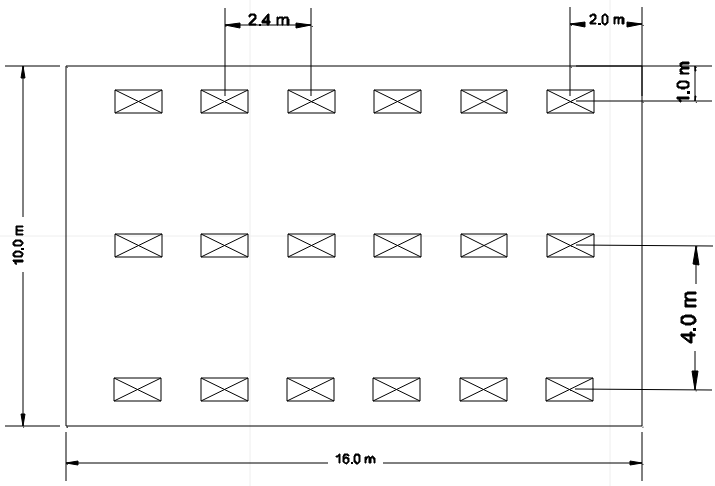
\includegraphics[width=0.6\textwidth]{lights}
\caption{Схема освещения помещения}
\label{pic:lights}
\end{figure}

Следовательно, светильники следует расположить в три ряда по шесть светильников, как показано на рисунке \ref{pic:lights}.

При этом имеет место избыточное освещение, превышающее расчетный световой поток на $(54-52) / 52=3.8\%$ (допустимым является 20\%
        отклонение).
Таким образом, в проекте используются $18$ светильников с высотой подвеса $0.1\ м$ и, соответственно, $54$ люминесцентных ламп
\textit{ЛБ-80} со
световым потоком $5220\ лм$ и световой отдачей $65.3\ лм/Вт$.

